\chapter{Resultados y discusión}
En este capítulo se presentan los resultados obtenidos de las simulaciones de transmisión de calor por conducción de un sistema TPV de un nano-espaciador y
radiación por campo cercano entre dos placas paralelas a 800°C el emisor y 25°C la célula. A su vez se representa las relaciones entre la potencia radiada vs la potencia conducida por cantidad de espaciadores y por distancia de separación en un sistema de emisor y célula de 1cm2.
\begin{itemize}
	\item Primero se comprueba si el procedimiento de extracción de datos de la simulación de transmisión de calor por conducción en CFD es adecuado y no presenta un error relativo significativo respecto a la teoría.
	\item Se presentan los resultados de las simulaciones de transmisión de calor por conducción y por radiación de campo cercano para diferentes combinaciones de materiales de emisor y célula, y la relación entre ambas simulaciones.
	\item Se estudia el número mínimo de espaciadores necesarios para soportar la carga de los emisores.
	\item Por último, se presentan los resultados de usar un nano-espaciador de $Si$ en vez de $SiO_2$ para emisores de $Si$ y $SS$.
\end{itemize}
%% COMPROBACIÓN DEL PROCEDIMIENTO DE EXTRACCIÓN DE RESULTADOS DE CFD
\section{Comprobación del procedimiento de extracción de resultados de CFD}
El procedimiento de extracción de resultados de CFD está definido en el punto \ref{it:extraerResCFD} del capítulo \ref{chapter:Metodos} y para su comprobación se procede a realizar una simulación en CFD donde el emisor y la célula son de $Si$ y el nano-espaciador de $SiO_2$ con las características constantes a 25\textdegree C, con la base cuadrada de 1 $mm^2$ y la altura del nano-espaciador a unos 1000nm, todo con la escalas correspondientes aplicadas.\\\\
La conductividad térmica ($\sigma$) del $Si$ es 182.977 W/m\textdegree C y la del $SiO_2$ es 1.30067 W/m\textdegree C ambas a 25\textdegree C. De la simulación se extrae que el flujo de calor del sistema y la temperatura media máxima y mínima de las superficies de contacto del nano-espaciador con los otros componentes del sistema.\\\\
La temperatura media máxima del nano-espaciador es 792.601\textdegree C, la temperatura media mínima del nano-espaciador es 32.3903\textdegree C y el flujo de calor es 0.00889793 W. Con los resultados de las temperaturas medias del nano-espaciador se obtiene un flujo de calor teórico de 0.00889905 W, obteniéndose un error relativo aproximado del 0.0126\%, por lo tanto el procedimiento es apropiado para la obtención de los resultados de las simulaciones de transmisión de calor por conducción.
%%% SIMULACIONES DE TRANSMISIÓN DE CALOR POR CONDUCCIÓN EN CFD
\section{Sistema TPV de Si-SiO2-Si}
Primero se estudia un caso sencillo de un sistema TPV de emisor y célula de $Si$, el efecto de la resistencia de contacto entre emisor y nano-espaciador sobre el flujo de calor y el efecto de la porosidad del $SiO_2$ del nano-espaciador en la potencia de conducción. En segundo lugar se estudia la relación entre la potencia radiada en un 1$cm^2$ de emisor y célula, y la potencia conducida.\\
\begin{figure}[H]
	\centering
	\begin{subfigure}[b]{0.49\textwidth}
		\centering
		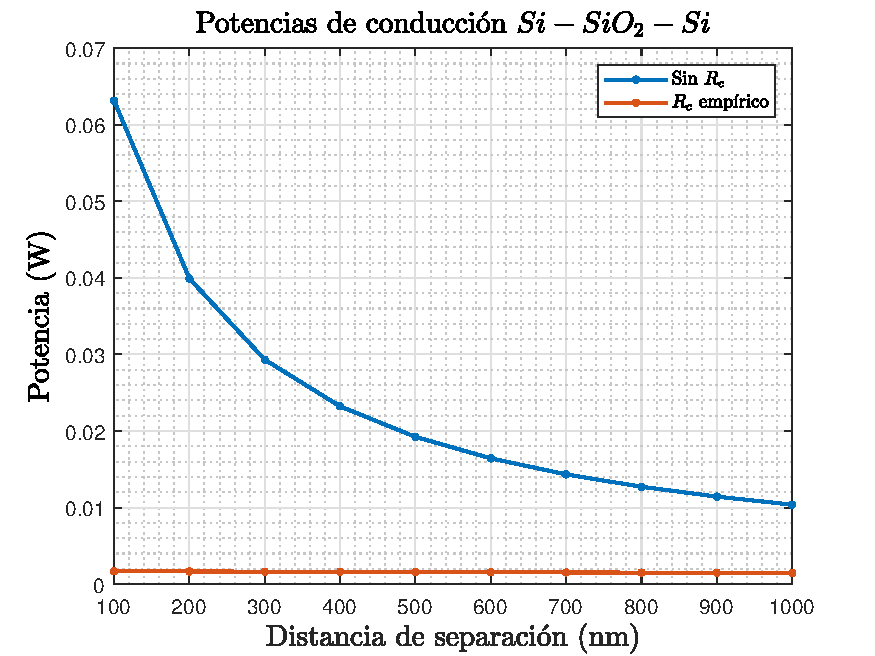
\includegraphics[width=1.0\textwidth]{figuras/Resultados/conduccion/pdf/Prc_SiSiO2Si.pdf}
		\caption{ }
		\label{fig:Prc_SiSiO2Si}
	\end{subfigure}
	\begin{subfigure}[b]{0.49\textwidth}
		\centering
		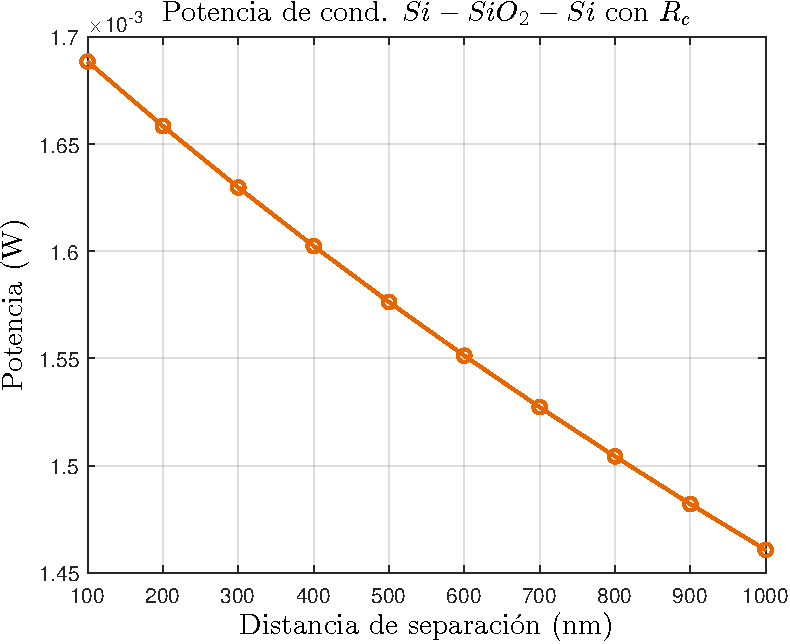
\includegraphics[width=1.0\textwidth]{figuras/Resultados/conduccion/pdf/Prc2_SiSiO2Si.pdf}
		\caption{ }
		\label{fig:Prc2_SiSiO2Si}
	\end{subfigure}
	\begin{subfigure}[b]{0.49\textwidth}
		\centering
		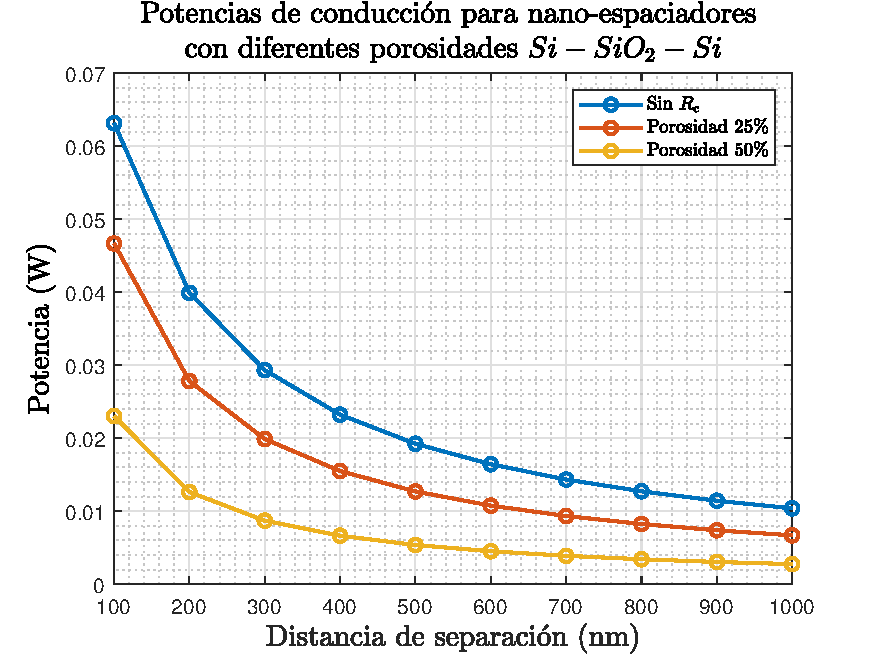
\includegraphics[width=1.0\textwidth]{figuras/Resultados/conduccion/pdf/Ppor_SiSiO2Si.pdf}
		\caption{ }
		\label{fig:Ppor_SiSiO2Si}
	\end{subfigure}
	\begin{subfigure}[b]{0.49\textwidth}
		\centering
		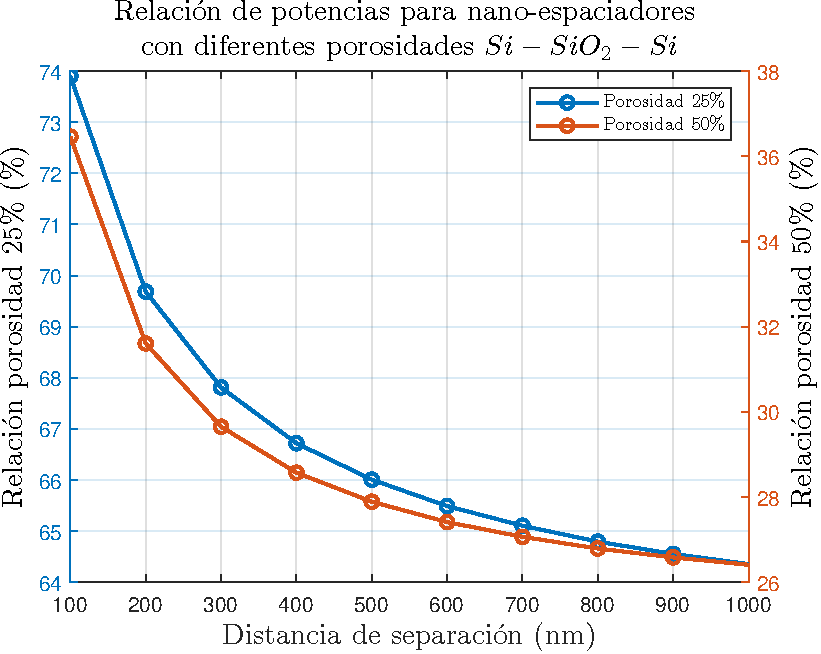
\includegraphics[width=1.0\textwidth]{figuras/Resultados/conduccion/pdf/relPpor_SiSiO2Si.pdf}
		\caption{ }
		\label{fig:relPpor_SiSiO2Si}
	\end{subfigure}
	\caption{ }
	\label{fig:Pcond_SiSiO2Si}
\end{figure}
\[Rel=\frac{\left| P_{Porosidad}- P_{Normal} \right|}{P_{Normal}}\cdot 100\]
\[P(d,p1(p),q1(p))=\frac{p1(p)}{d+q1(p)}\]
\[p1(p)=-16.47\cdot p +11.03 \ q1(p)=-106.80\cdot p+74.68\]
\[P(d,p)=\frac{  16.47\cdot p-11.03 }{d-106.80\cdot p +74.68}\]
\subsection{Efectos de la resistencia de contacto}

De las simulaciones de transmisión de calor de CFD, se obtienen los siguientes resultados:
\begin{table}[H]
	\centering
		\begin{tabular}{|c||c|c|c|c||c|c|}
		\hline
			\multirow{2}{*}{ }& \multicolumn{6}{c|}{\textbf{\large Potencias según como se transmite el calor}}\\ \cline{2-7}
		  & \multicolumn{4}{c||}{Conducción (W/nº nano-espaciadores)}& \multicolumn{2}{c|}{Radiación $(W/m^2)$}\\ \hline
			Dist. (nm)&$P_{Normal}$&$P_{R_c-Empirico}$&$P_{Porosidad25}$&$P_{Porosidad50}$&$P_{Eg>0.7eV}$&$P_{full}$\\ \hline \hline
			100&6,31E-02&1,69E-03&4,67E-02&2,30E-02&5,07E+03&1,65E+05\\ \hline
			200&3,99E-02&1,66E-03&2,78E-02&1,26E-02&3,11E+03&1,10E+05\\ \hline
			300&2,93E-02&1,63E-03&1,99E-02&8,69E-03&2,30E+03&8,51E+04\\ \hline
			400&2,32E-02&1,60E-03&1,55E-02&6,63E-03&1,90E+03&7,01E+04\\ \hline
			500&1,92E-02&1,58E-03&1,27E-02&5,36E-03&1,70E+03&6,02E+04\\ \hline
			600&1,64E-02&1,55E-03&1,08E-02&4,50E-03&1,66E+03&5,32E+04\\ \hline
			700&1,43E-02&1,53E-03&9,33E-03&3,88E-03&1,72E+03&4,80E+04\\ \hline
			800&1,27E-02&1,50E-03&8,24E-03&3,41E-03&1,82E+03&4,43E+04\\ \hline
			900&1,14E-02&1,48E-03&7,38E-03&3,04E-03&1,86E+03&4,14E+04\\ \hline
			1000&1,04E-02&1,46E-03&6,68E-03&2,74E-03&1,80E+03&3,93E+04\\ \hline
		\end{tabular}
	\caption{Tabla de resultados de las simulaciones de conducción y radiación de campo cercano para diferentes alturas del nano-espaciador. Flujos de calor del TPV $Si-SiO_2-Si$ para diferentes alturas del nano-espaciador y para los casos sin $R_c$, con $R_c$ de \cite{nf_TPV_Pillars_SiO2}, sin $R_c$ pero con las proporciones de las porosidades de \cite{ThermalConductivity_SiO2_2018} para un 25\% y un 50\%.}
	\label{tab:condTerSiSiO2Si}
\end{table}
\begin{figure}[H]
	\centering
	%% Si-SiO2-Si Eg
	\begin{subfigure}[b]{0.49\textwidth}
		\centering
		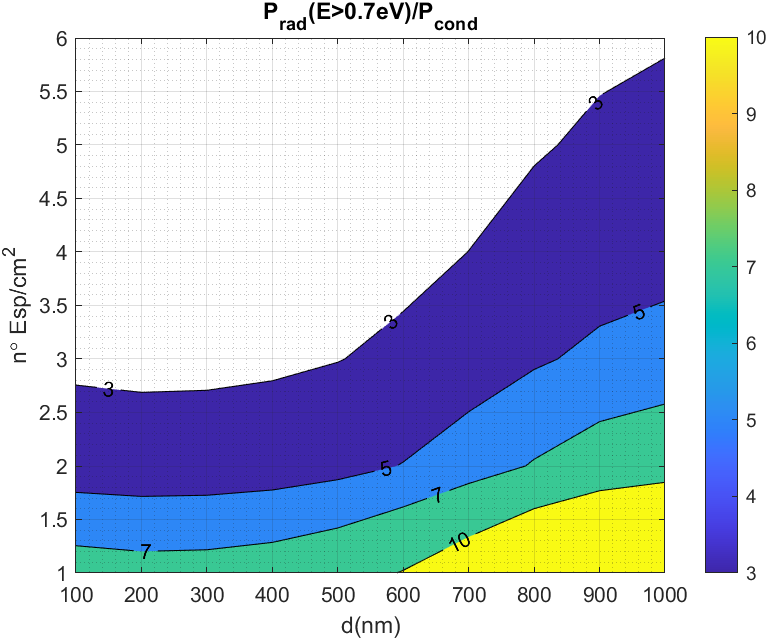
\includegraphics[width=1.00\textwidth]{figuras/Resultados/RelacionCondRad/SiSi.png}
		\caption{ }
		\label{fig:rel_SiSiO2Si}
	\end{subfigure}
	\hfill
	\begin{subfigure}[b]{0.49\textwidth}
		\centering
		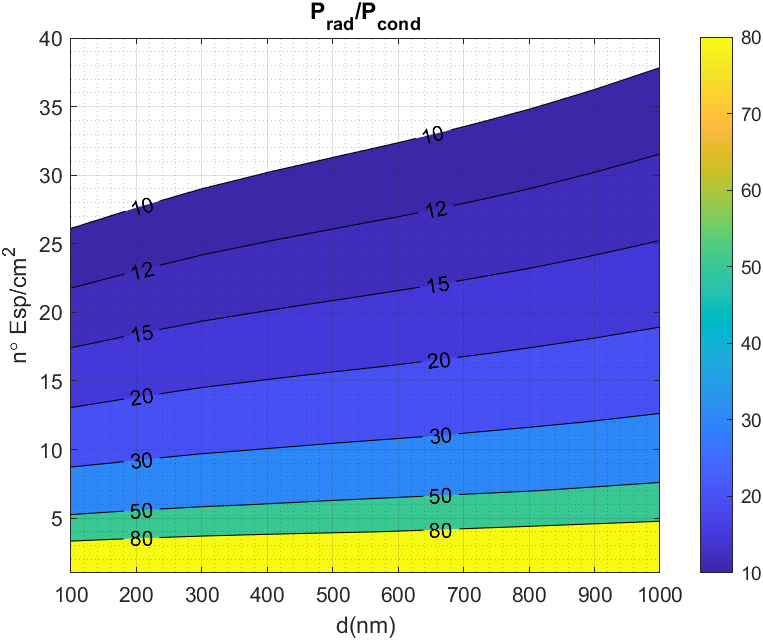
\includegraphics[width=1.00\textwidth]{figuras/Resultados/RelacionCondRad/SiSi_full.png}
		\caption{ }
		\label{fig:rel_SiSiO2Si_full}
	\end{subfigure}
	\hfill
	\begin{subfigure}[b]{0.49\textwidth}
		\centering
		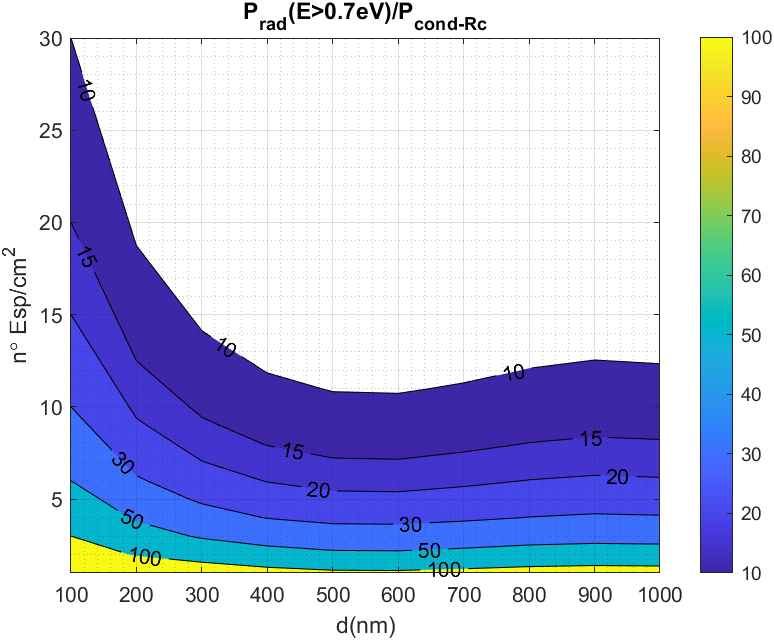
\includegraphics[width=1.00\textwidth]{figuras/Resultados/RelacionCondRad/SiSi_Rc.png}
		\caption{ }
		\label{fig:rel_SiSiO2Si_Rc}
	\end{subfigure}
	\hfill
	\begin{subfigure}[b]{0.49\textwidth}
		\centering
		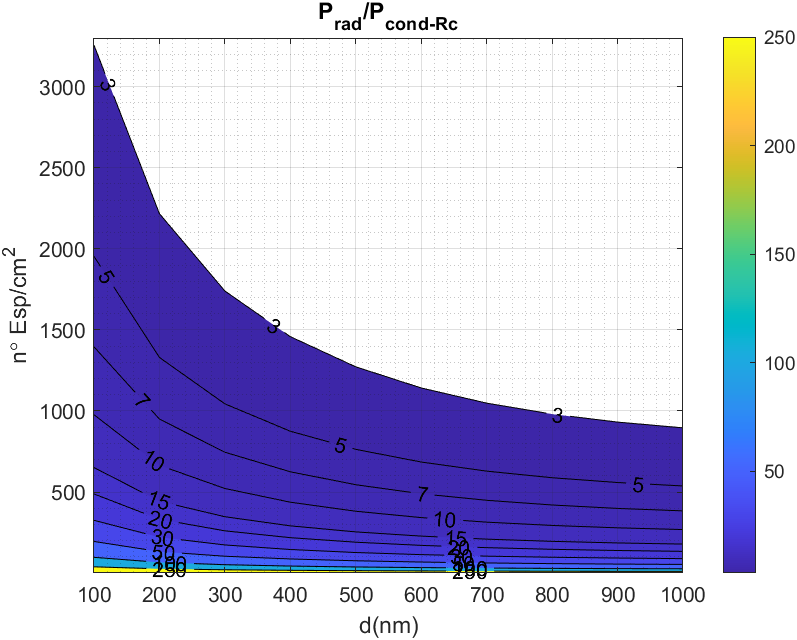
\includegraphics[width=1.00\textwidth]{figuras/Resultados/RelacionCondRad/SiSi_Rc_full.png}
		\caption{ }
		\label{fig:rel_SiSiO2Si_Rc_full}
	\end{subfigure}
	\caption{ }
	\label{fig:relation_SiSiO2Si}
\end{figure}

\begin{figure}[H]
	\centering
	%% Si-SiO2-Si Eg
	\begin{subfigure}[b]{0.49\textwidth}
		\centering
		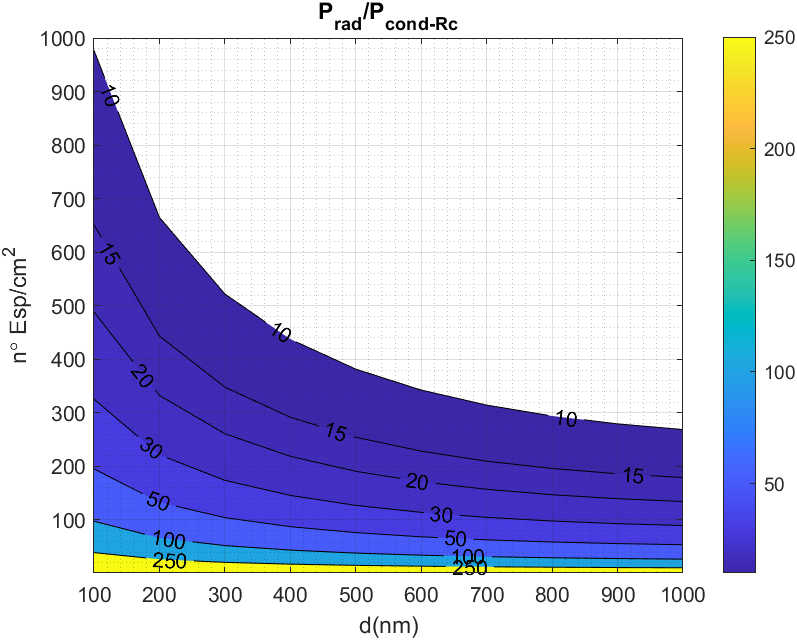
\includegraphics[width=1.00\textwidth]{figuras/Resultados/RelacionCondRad/SiSi_Rc_full_10.png}
		\caption{ }
		\label{fig:rel_SiSiO2Si_Rc_full_10}
	\end{subfigure}
	\hfill
	\begin{subfigure}[b]{0.49\textwidth}
		\centering
		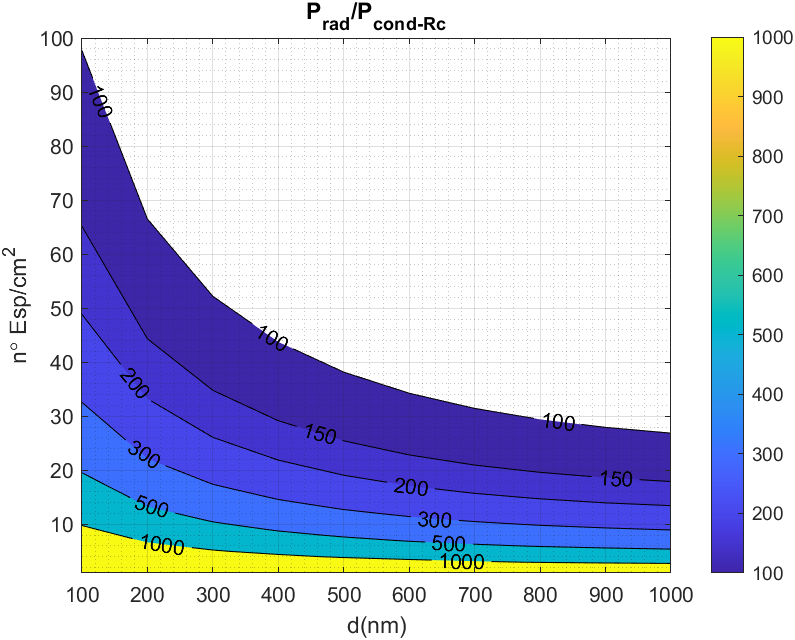
\includegraphics[width=1.00\textwidth]{figuras/Resultados/RelacionCondRad/SiSi_Rc_full_100.png}
		\caption{ }
		\label{fig:rel_SiSiO2Si_Rc_full_100}
	\end{subfigure}
	\caption{ }
	\label{fig:relation_SiSiO2Si_zoomIn}
\end{figure}

\section{Caso 2: Sistema TPV de $Si-SiO_2-Ge$}
\begin{table}[h]
	\centering
		\begin{tabular}{|c|c|c|}
		\hline
			dnm&Pn&Prcpaper \\ \hline 
100&5,38E-02&1,68E-03 \\ \hline 
200&3,65E-02&1,65E-03 \\ \hline 
300&2,76E-02&1,62E-03 \\ \hline 
400&2,22E-02&1,60E-03 \\ \hline 
500&1,85E-02&1,57E-03 \\ \hline 
600&1,59E-02&1,55E-03 \\ \hline 
700&1,39E-02&1,52E-03 \\ \hline 
800&1,24E-02&1,50E-03 \\ \hline 
900&1,12E-02&1,48E-03 \\ \hline 
1000&1,02E-02&1,46E-03 \\ \hline 
		\end{tabular}
	\caption{cs}
	\label{tab:cs}
\end{table}
\begin{figure}[H]
	\centering
	%% Si-SiO2-Si Eg
	\begin{subfigure}[b]{0.49\textwidth}
		\centering
		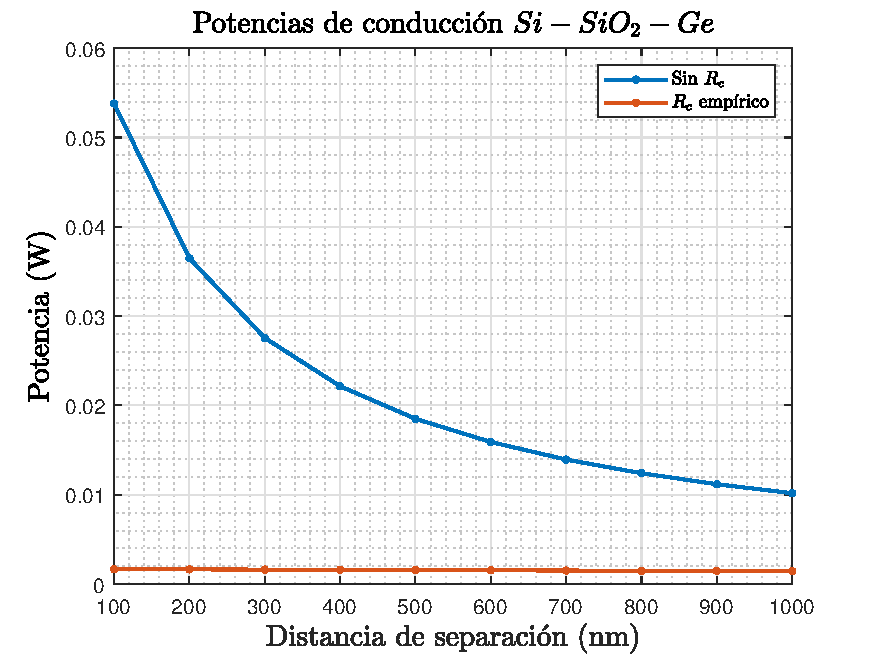
\includegraphics[width=1.00\textwidth]{figuras/Resultados/conduccion/pdf/Prc_SiSiO2Ge.pdf}
		\caption{ }
		\label{fig:Prc_SiSiO2Ge}
	\end{subfigure}
	\hfill
	\begin{subfigure}[b]{0.49\textwidth}
		\centering
		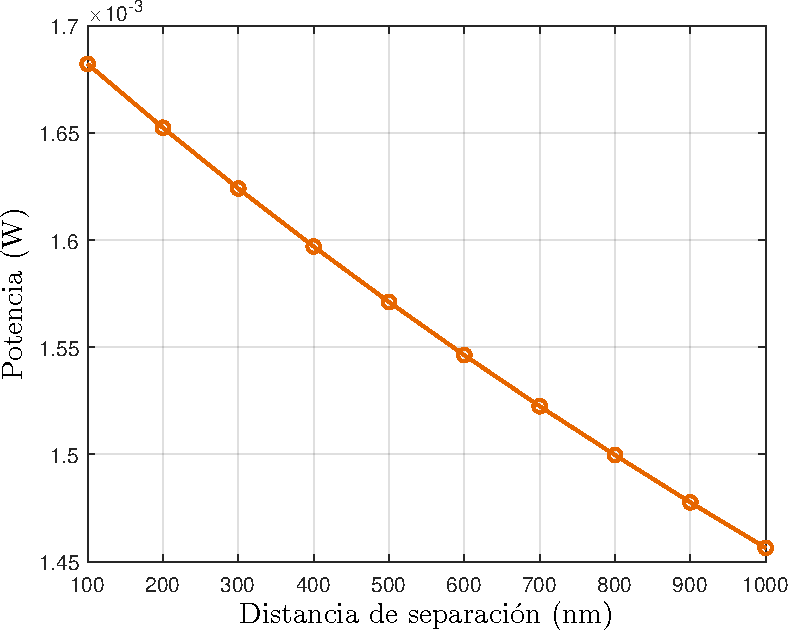
\includegraphics[width=1.00\textwidth]{figuras/Resultados/conduccion/pdf/Prc2_SiSiO2Ge.pdf}
		\caption{ }
		\label{fig:Prc2_SiSiO2Ge}
	\end{subfigure}
	\caption{ }
	\label{fig:Pcond_SiSiO2Ge}
\end{figure}

\begin{figure}[H]
	\centering
	%% Si-SiO2-Si Eg
	\begin{subfigure}[b]{0.49\textwidth}
		\centering
		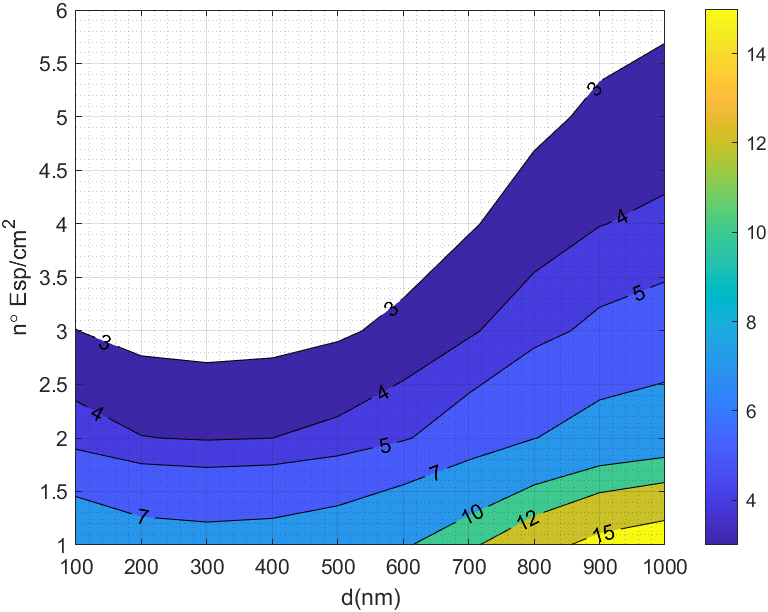
\includegraphics[width=1.00\textwidth]{figuras/Resultados/RelacionCondRad/SiGe.png}
		\caption{ }
		\label{fig:rel_SiSiO2Ge}
	\end{subfigure}
	\hfill
	\begin{subfigure}[b]{0.49\textwidth}
		\centering
		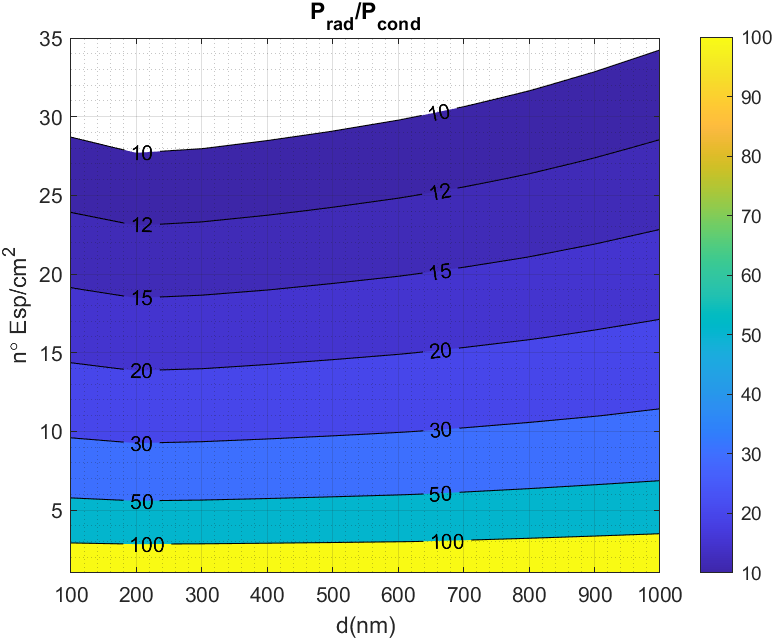
\includegraphics[width=1.00\textwidth]{figuras/Resultados/RelacionCondRad/SiGe_full.png}
		\caption{ }
		\label{fig:rel_SiSiO2Ge_full}
	\end{subfigure}
	\hfill
	\begin{subfigure}[b]{0.49\textwidth}
		\centering
		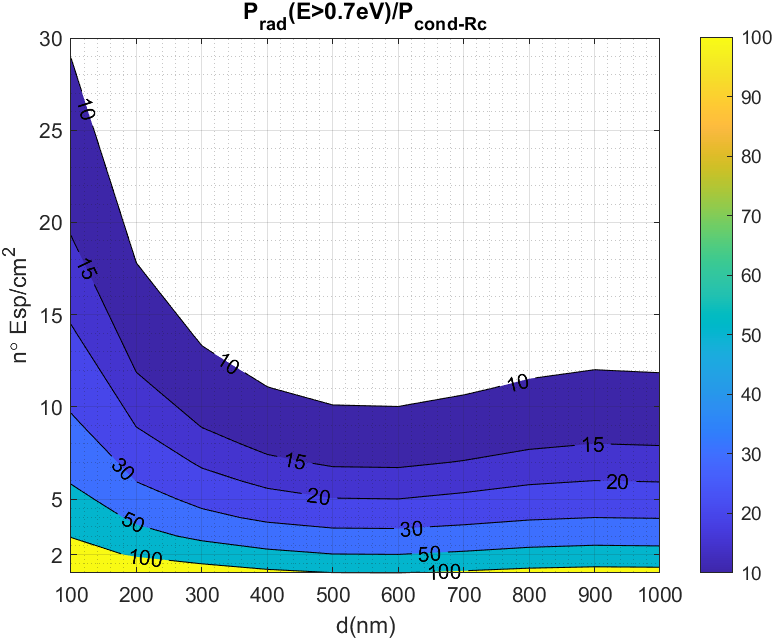
\includegraphics[width=1.00\textwidth]{figuras/Resultados/RelacionCondRad/SiGe_Rc.png}
		\caption{ }
		\label{fig:rel_SiSiO2Ge_Rc}
	\end{subfigure}
	\hfill
	\begin{subfigure}[b]{0.49\textwidth}
		\centering
		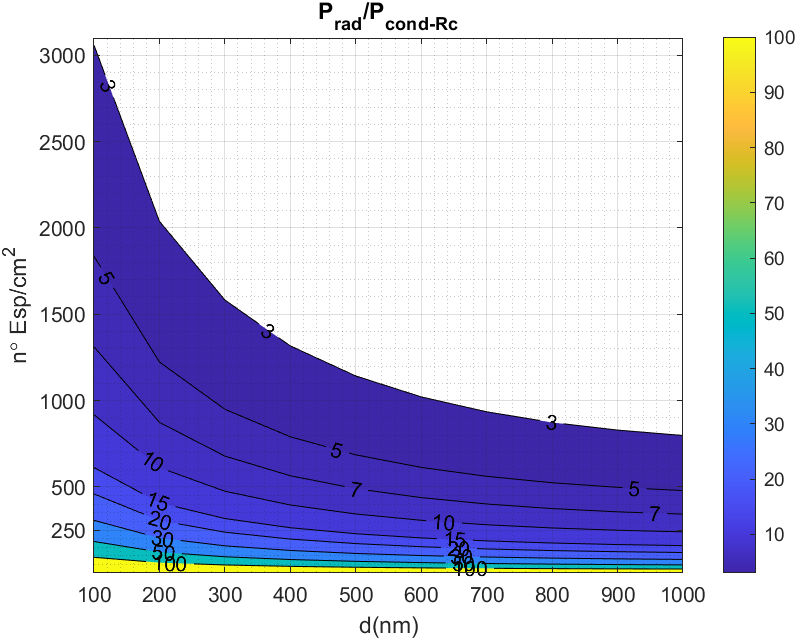
\includegraphics[width=1.00\textwidth]{figuras/Resultados/RelacionCondRad/SiGe_Rc_full.png}
		\caption{ }
		\label{fig:rel_SiSiO2Ge_Rc_full}
	\end{subfigure}
	\caption{ }
	\label{fig:relation_SiSiO2Ge}
\end{figure}

\begin{figure}[H]
	\centering
	%% Si-SiO2-Si Eg
	\begin{subfigure}[b]{0.49\textwidth}
		\centering
		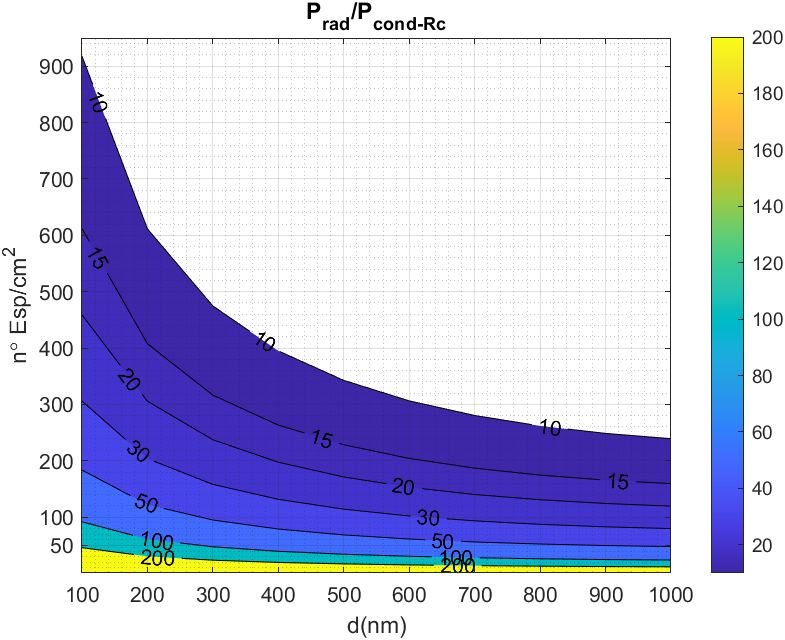
\includegraphics[width=1.00\textwidth]{figuras/Resultados/RelacionCondRad/SiGe_Rc_full_10.png}
		\caption{ }
		\label{fig:rel_SiSiO2Ge_Rc_full_10}
	\end{subfigure}
	\hfill
	\begin{subfigure}[b]{0.49\textwidth}
		\centering
		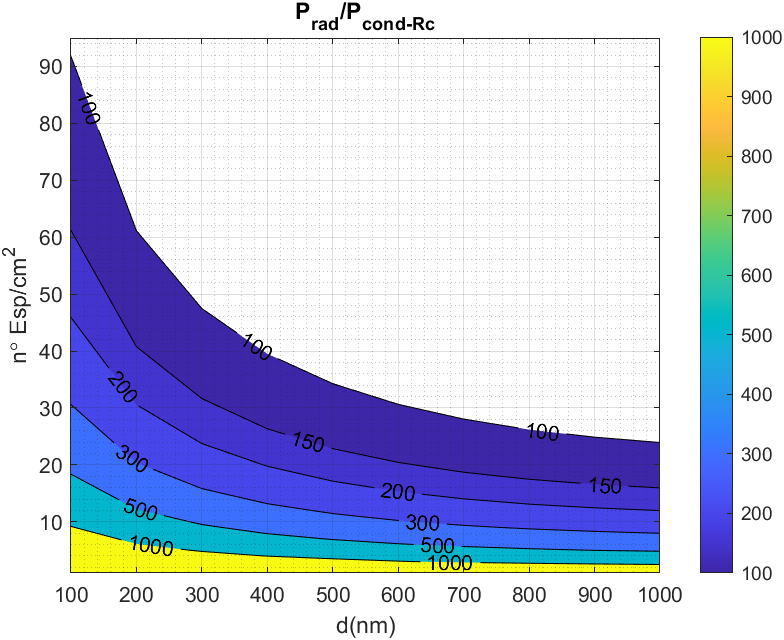
\includegraphics[width=1.00\textwidth]{figuras/Resultados/RelacionCondRad/SiGe_Rc_full_100.png}
		\caption{ }
		\label{fig:rel_SiSiO2Ge_Rc_full_100}
	\end{subfigure}
	\caption{ }
	\label{fig:relation_SiSiO2Ge_zoomIn}
\end{figure}
\section{Caso 3: Sistema TPV de $SS-SiO_2-Ge$}
\begin{table}[h]
	\centering
		\begin{tabular}{|c|c|c|c|c|}
		\hline
			dnm&Pn&Prcmax&Prcinter&Prcpaper \\ \hline 
100&4,79578E-02&1,26815E-06&2,53438E-06&1,67993E-03 \\ \hline 
200&3,41638E-02&1,26813E-06&2,53431E-06&1,65024E-03 \\ \hline 
300&2,64074E-02&1,26811E-06&2,53424E-06&1,62198E-03 \\ \hline 
400&2,14795E-02&1,26809E-06&2,53417E-06&1,59500E-03 \\ \hline 
500&1,80787E-02&1,26808E-06&2,53410E-06&1,56919E-03 \\ \hline 
600&1,56074E-02&1,26806E-06&2,53403E-06&1,54444E-03 \\ \hline 
700&1,37190E-02&1,26804E-06&2,53396E-06&1,52066E-03 \\ \hline 
800&1,22454E-02&1,26802E-06&2,53388E-06&1,49795E-03 \\ \hline 
900&1,10504E-02&1,26800E-06&2,53381E-06&1,47593E-03 \\ \hline 
1000&1,00695E-02&1,26799E-06&2,53374E-06&1,45476E-03 \\ \hline
		\end{tabular}
	\caption{daa}
	\label{tab:daa}
\end{table}
\begin{figure}[H]
	\centering
	\begin{subfigure}[b]{0.49\textwidth}
		\centering
			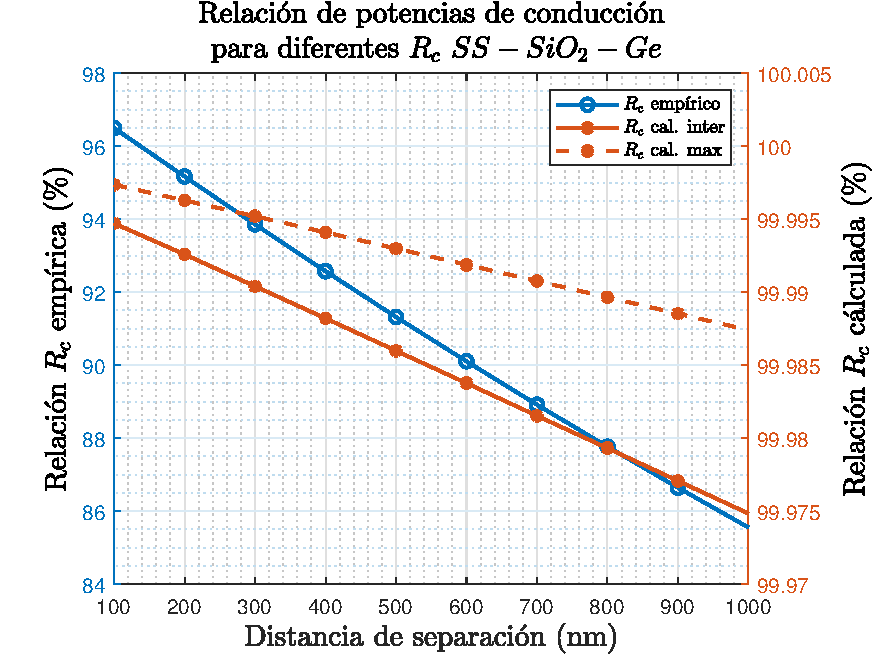
\includegraphics[width=1.00\textwidth]{figuras/Resultados/conduccion/pdf/relPrcs_SsSiO2Ge.pdf}
		\caption{ }
		\label{fig:relPrcs_SsSiO2Ge}
	\end{subfigure}
	\hfill
	\begin{subfigure}[b]{0.49\textwidth}
		\centering
			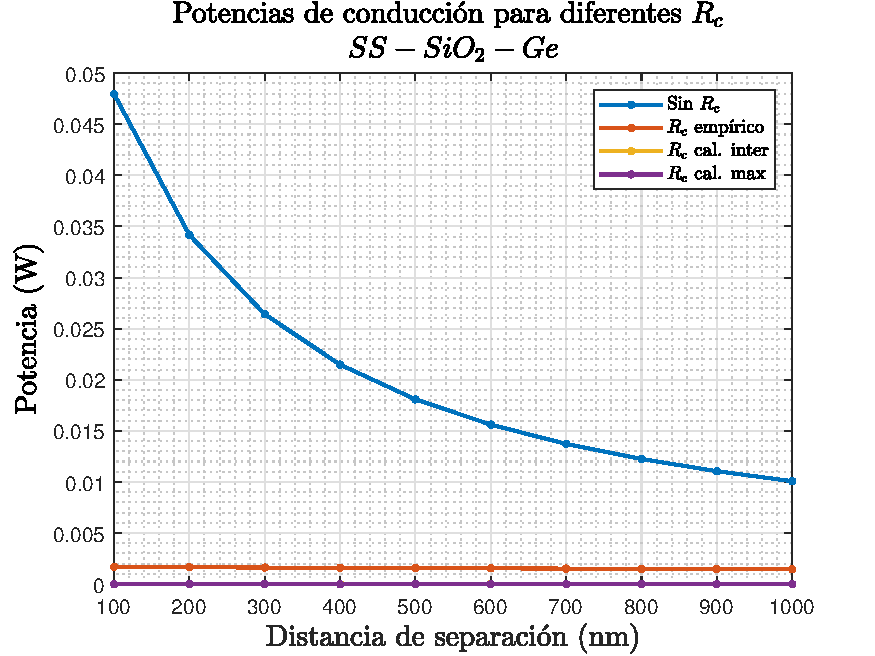
\includegraphics[width=1.00\textwidth]{figuras/Resultados/conduccion/pdf/Prcs_SsSiO2Ge.pdf}
		\caption{ }
		\label{fig:Prcs_SsSiO2Ge}
	\end{subfigure}
	\caption{ }
	\label{fig:Pcond_SsSiO2Ge}
\end{figure}

\begin{figure}[H]
	\centering
	\begin{subfigure}[b]{0.49\textwidth}
		\centering
			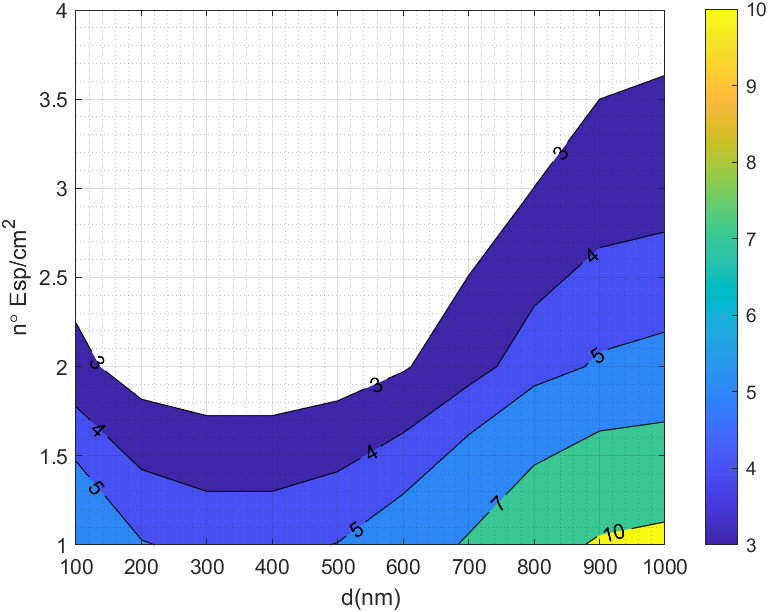
\includegraphics[width=1.00\textwidth]{figuras/Resultados/RelacionCondRad/SS.png}
		\caption{ }
		\label{fig:rel_SsSiO2Ge}
	\end{subfigure}
	\hfill
	\begin{subfigure}[b]{0.49\textwidth}
		\centering
			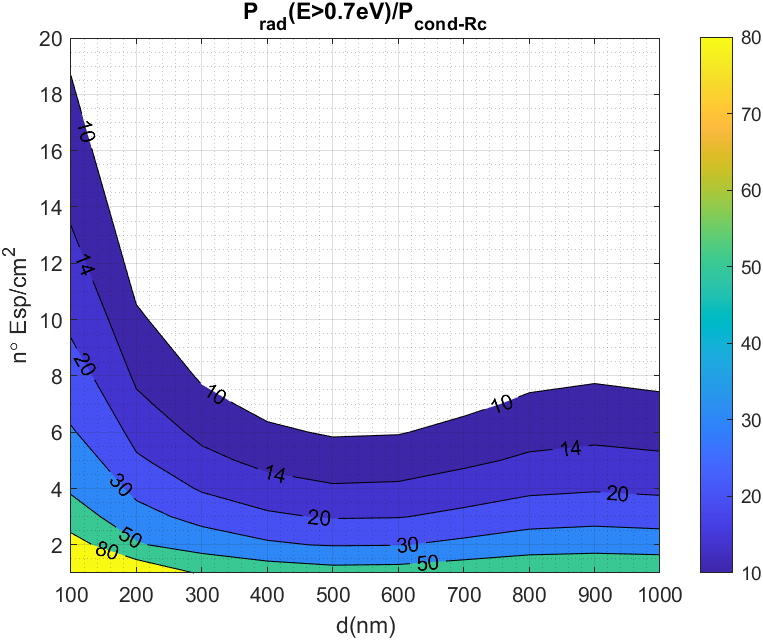
\includegraphics[width=1.00\textwidth]{figuras/Resultados/RelacionCondRad/SS_Rc_empirico.png}
		\caption{ empirico}
		\label{fig:rel_SsSiO2Ge_Rc_emp}
	\end{subfigure}
	\hfill
	\begin{subfigure}[b]{0.49\textwidth}
		\centering
			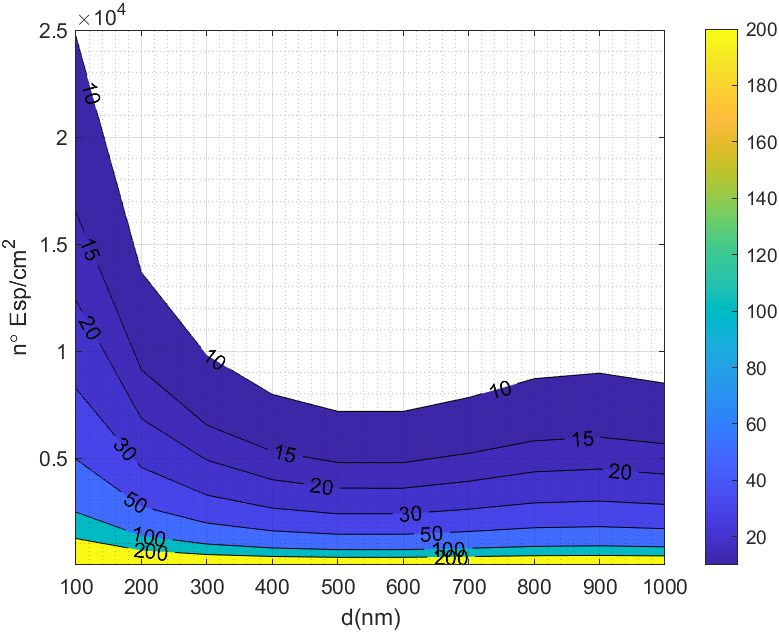
\includegraphics[width=1.00\textwidth]{figuras/Resultados/RelacionCondRad/SS_Rc.png}
		\caption{ max}
		\label{fig:rel_SsSiO2Ge_Rc_max}
	\end{subfigure}
	\hfill
	\begin{subfigure}[b]{0.49\textwidth}
		\centering
			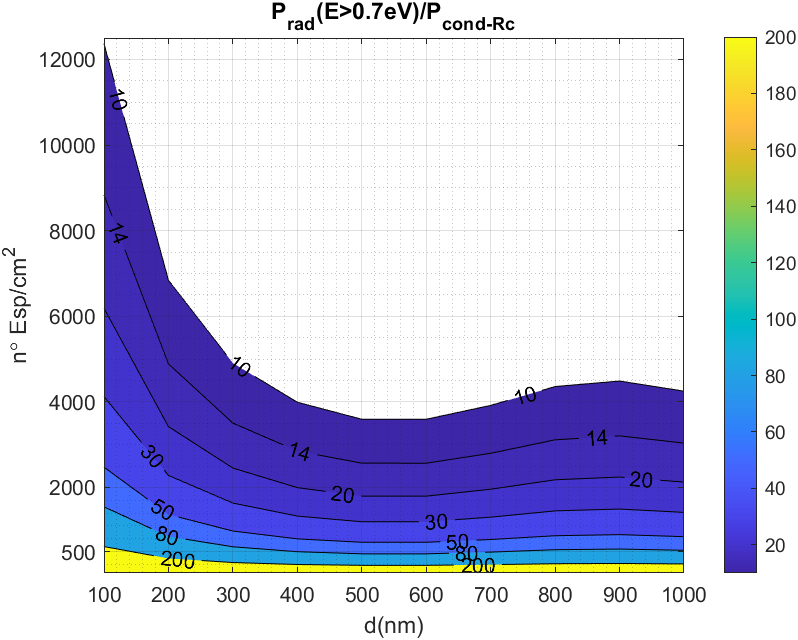
\includegraphics[width=1.00\textwidth]{figuras/Resultados/RelacionCondRad/SS_Rc_Intermedio.png}
		\caption{ intermedio}
		\label{fig:rel_SsSiO2Ge_Rc_inter}
	\end{subfigure}
	\caption{ }
	\label{fig:relation_SsSiO2Ge}
\end{figure}

\begin{figure}[H]
	\centering
	%% Si-SiO2-Si Eg
	\begin{subfigure}[b]{0.49\textwidth}
		\centering
		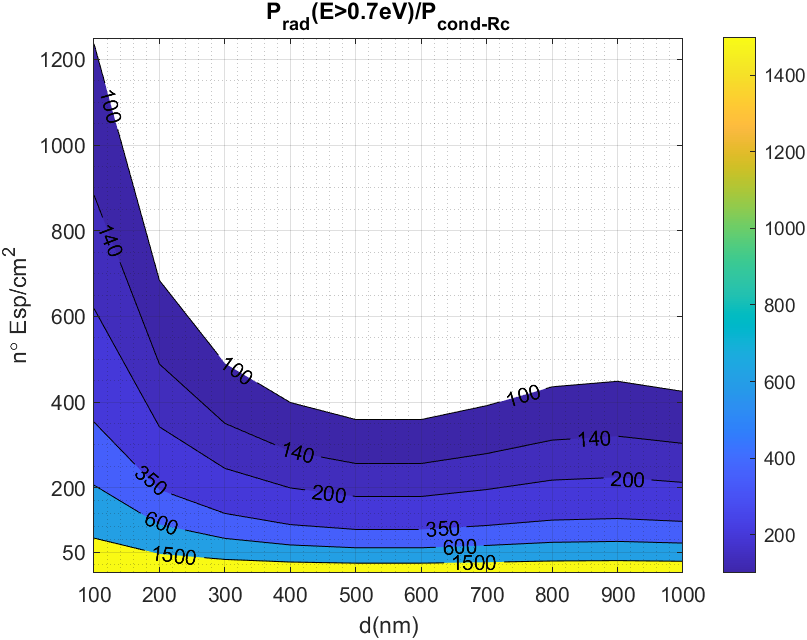
\includegraphics[width=1.00\textwidth]{figuras/Resultados/RelacionCondRad/SS_Rc_Intermedio_100.png}
		\caption{intermedio }
		\label{fig:rel_SsSiO2Ge_Rc_inter_100}
	\end{subfigure}
	\hfill
	\begin{subfigure}[b]{0.49\textwidth}
		\centering
		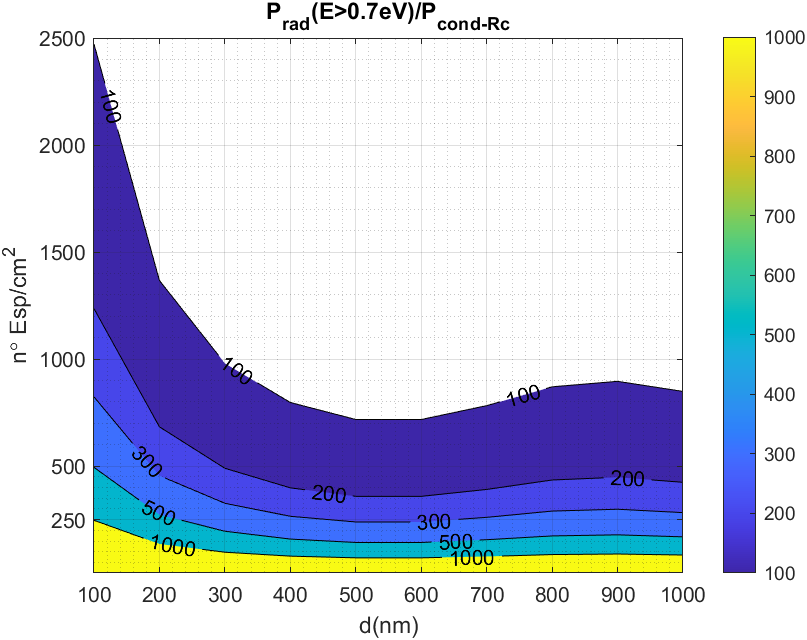
\includegraphics[width=1.00\textwidth]{figuras/Resultados/RelacionCondRad/SS_Rc_100s.png}
		\caption{ }
		\label{fig:rel_SsSiO2Ge_Rc_max_100}
	\end{subfigure}
	\caption{ }
	\label{fig:rel_SsSiO2Ge_100}
\end{figure}
%%% 
\section{Caso 4: Sistema TPV de $SiC-SiO_2-Ge$}
\begin{table}[h]
	\centering
		\begin{tabular}{|c|c|c|}
		\hline
			dnm&Pn&Prc\\ \hline 
100&6,23E-02&1,69E-03\\ \hline 
200&4,09E-02&1,66E-03\\ \hline 
300&3,03E-02&1,63E-03\\ \hline 
400&2,39E-02&1,61E-03\\ \hline 
500&1,98E-02&1,58E-03\\ \hline 
600&1,68E-02&1,55E-03\\ \hline 
700&1,47E-02&1,53E-03\\ \hline 
800&1,30E-02&1,51E-03\\ \hline 
900&1,17E-02&1,49E-03\\ \hline 
1000&1,06E-02&1,46E-03\\ \hline 
		\end{tabular}
	\caption{dac}
	\label{tab:dac}
\end{table}

relleno
\begin{figure}[H]
	\centering
		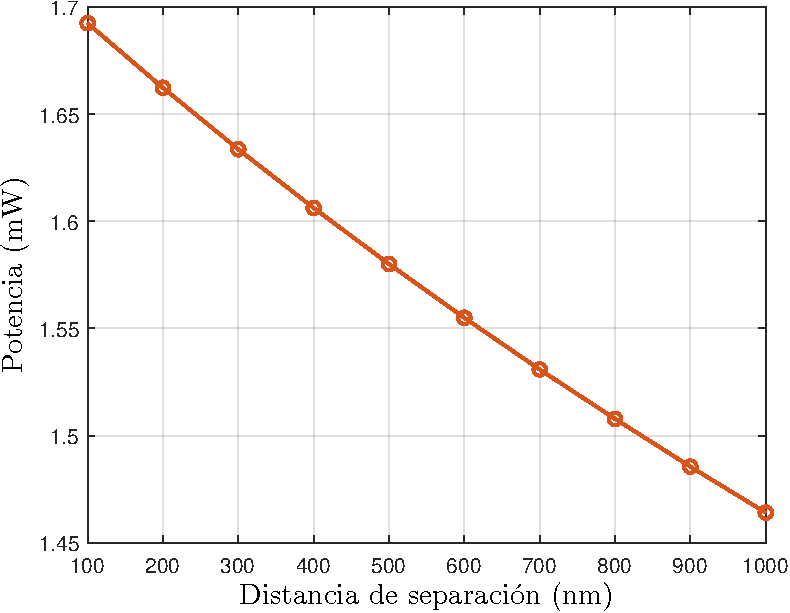
\includegraphics[width=0.6\textwidth]{figuras/Resultados/conduccion/pdf/Prc_SiCSiO2Ge.pdf}
	\caption{ }
	\label{fig:Prc_SiCSiO2Ge}
\end{figure}

\begin{figure}[H]
	\centering
	%% Si-SiO2-Si Eg
	\begin{subfigure}[b]{0.49\textwidth}
		\centering
		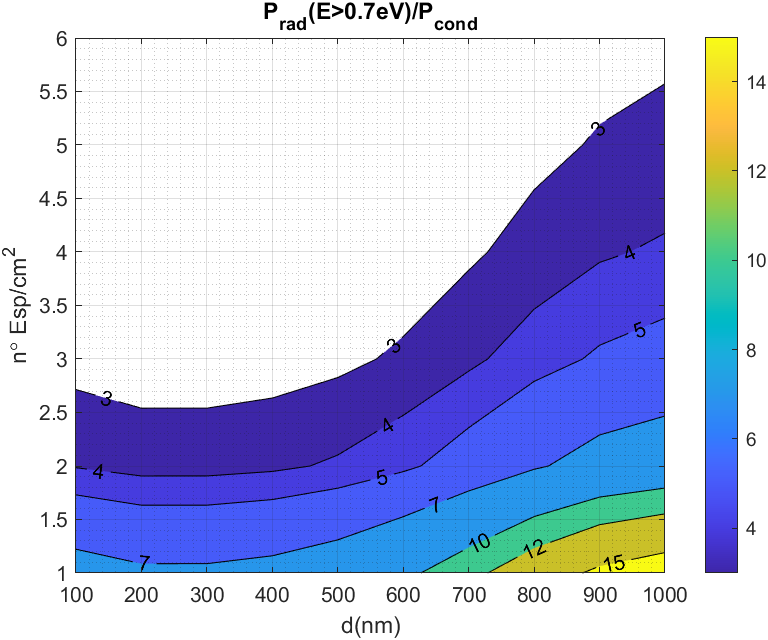
\includegraphics[width=1.00\textwidth]{figuras/Resultados/RelacionCondRad/SiC_Ge.png}
		\caption{ }
		\label{fig:rel_SiCSiO2Ge}
	\end{subfigure}
	\hfill
	\begin{subfigure}[b]{0.49\textwidth}
		\centering
		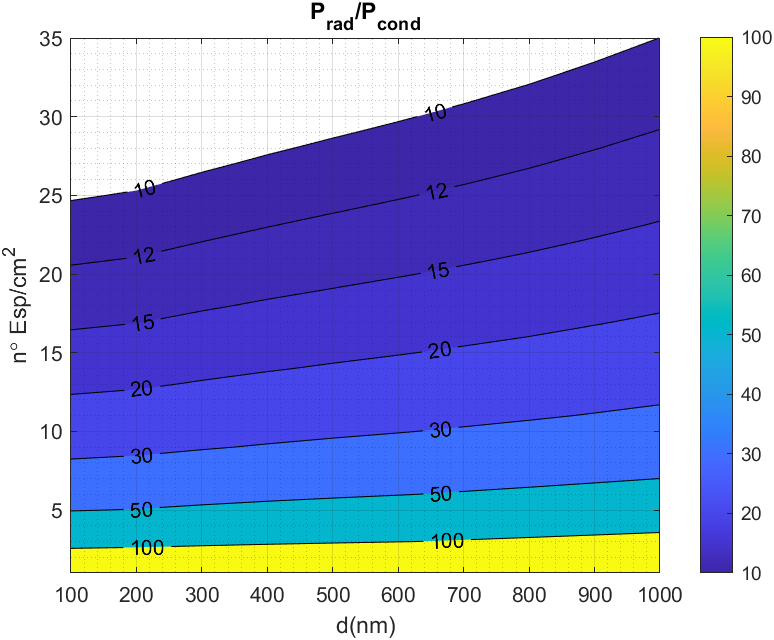
\includegraphics[width=1.00\textwidth]{figuras/Resultados/RelacionCondRad/SiC_Ge_full.png}
		\caption{ }
		\label{fig:rel_SiCSiO2Ge_Rc}
	\end{subfigure}
	\hfill
	\begin{subfigure}[b]{0.49\textwidth}
		\centering
		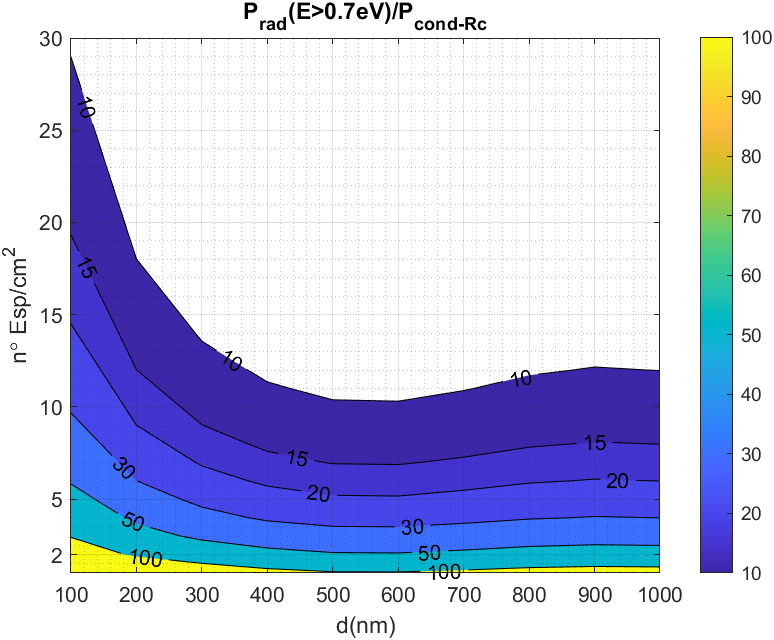
\includegraphics[width=1.00\textwidth]{figuras/Resultados/RelacionCondRad/SiC_Rc.png}
		\caption{ }
		\label{fig:rel_SiCSiO2Ge_full}
	\end{subfigure}
	\hfill
	\begin{subfigure}[b]{0.49\textwidth}
		\centering
		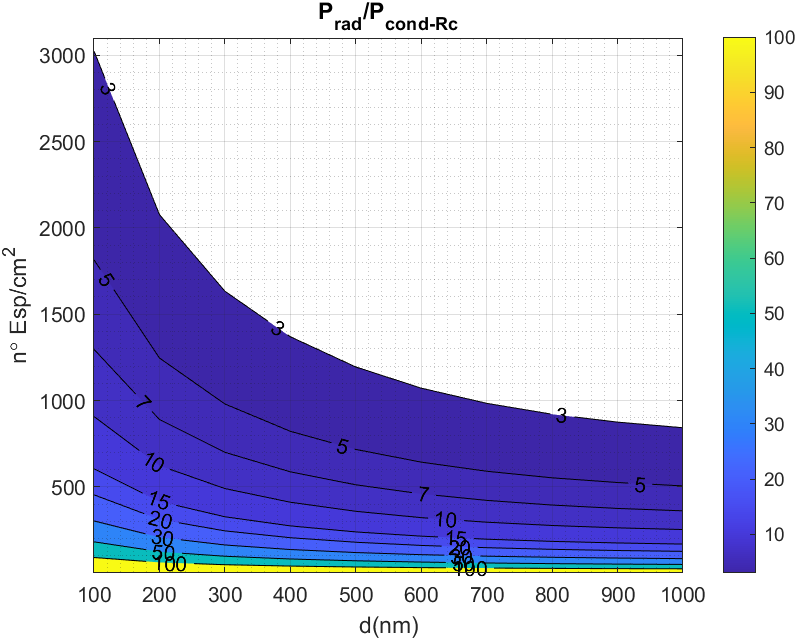
\includegraphics[width=1.00\textwidth]{figuras/Resultados/RelacionCondRad/SiC_Ge_Rc_full.png}
		\caption{ }
		\label{fig:rel_SiCSiO2Ge_Rc_full}
	\end{subfigure}
	\caption{ }
	\label{fig:relation_SiCSiO2Ge}
\end{figure}

\section{Resultados}

\begin{table}[H]
	\centering
		\begin{tabular}{|c|c|c|}
		\hline
		dnm&Prcpaper&Prc\_SS\\ \hline 
		100&0,0017136&0,00171126\\ \hline 
		200&0,0017135&0,00171117\\ \hline 
		300&0,00171336&0,00171103\\ \hline 
		400&0,00171322&0,00171089\\ \hline 
		500&0,00171304&0,00171072\\ \hline 
		600&0,00171282&0,0017105\\ \hline 
		700&0,00171257&0,00171025\\ \hline 
		800&0,0017125&0,00171019\\ \hline 
		900&0,0017122&0,00170989\\ \hline 
		1000&0,00171208&0,00170978\\ \hline
		\end{tabular}
	\caption{nano-espaciador de Si}
	\label{tab:nanoEspaciadorDeSi}
\end{table}

\section{Discusión}